\subsection{Configure FFTs}
\label{sec:ui_configure_ffts}

This dialog allows management of fixed field transponders (FFTs), as stored in the configuration as well as in the database. \\

\begin{figure}[H]
    \hspace*{-2cm}
    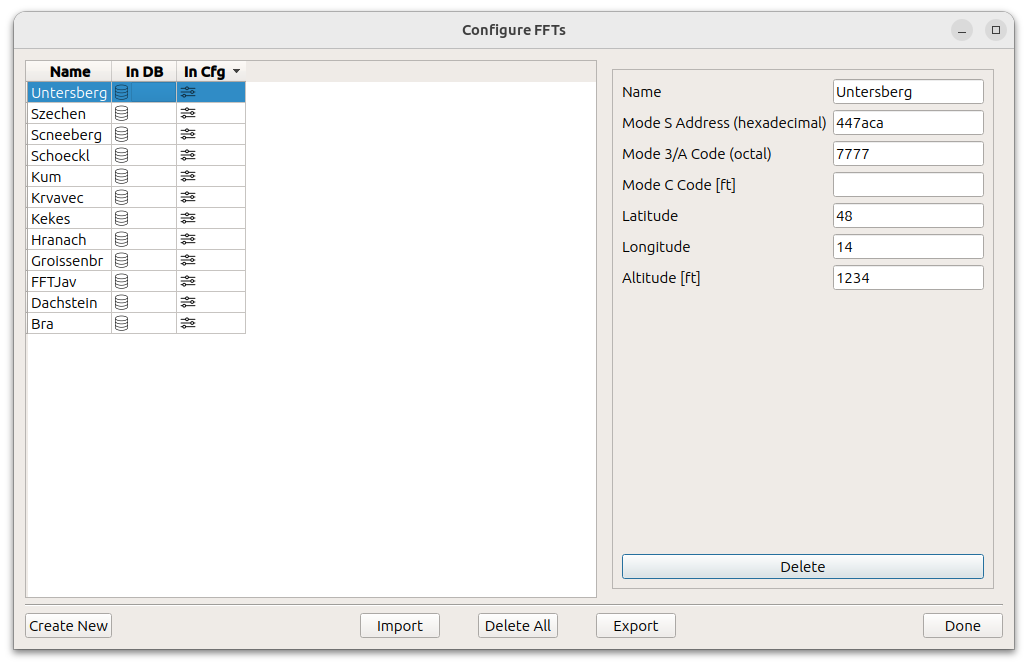
\includegraphics[width=18cm]{figures/configure_ffts.png}
  \caption{Configure Data Sources}
\end{figure}

The defined FFTs are used for:
\begin{itemize}
\item Display in Geographic View
\item Usage of correct altitude information for Radar slant range correction during ASTERIX import
\end{itemize}
\ \\

All FFTs are always stored in the configuration as well as in the database, which means it is persistent and can be used in all new databases. It is useful to define all existing FFTs, since they are immediately used during import of data. \\

\paragraph {FFT Table Content}
\label{sec:configure_ffts_table_content}

\begin{itemize}
\item Name: Name of the data source
\item Mode S Address (hexadecimal): Optional
\item Mode 3/A Code (octal): Optional
\item Mode C Code [ft]: Optional
\item Latitude, Longitude: WGS84 position in degrees
\item Altitude [ft]: Altitude above MSL, in feet
\end{itemize}
\ \\

\subsubsection{Import/Export of FFTs}
\label{sec:config_fft_export}

Using the 4 buttons on the bottom the following functions can be used:

\begin{itemize}
\item Create New: Create new FFT
\item Import: Import configuration FFTs from JSON file
\item Delete All: Delete all configuration FFTs
\item Export: Export all configuration FFTs as JSON file
\end{itemize}
\ \\

Using these functions, the configuration FFTs can be changed for sensor context switches, or e.g. exported before a COMPASS version upgrade.
